\documentclass[12pt]{report}
\newcommand{\version}{Draft: 24 August 2020}

\usepackage[reqno,intlimits,sumlimits,centertags]{amsmath}  % principal package in the AMS-LATEX distribution
\usepackage{amssymb}                                        % defines all the symbols found in the AMS symbol fonts msam and msbm
\usepackage{amsthm}                                         % facilitates the AMS theorem setup
\usepackage[title]{appendix}                                % provides various ways of formatting the titles of appendices
\usepackage[english]{babel}                                 % manages culturally determined typographical (and other) rules
\usepackage[plain]{fancyref}                                % fancy cross-referencing support
\usepackage{fancyhdr}                                       % construct headers and footers
\usepackage{fancyvrb}                                       % flexible handling of verbatim text
\usepackage[pdftex]{graphicx}                               % the ‘extended’ or ‘enhanced’ graphics package
\usepackage[utf8]{inputenc}                                 % accept different input encodings
\usepackage{natbib}                                         % author-year and numerical citations
\usepackage{rotating}                                       % perform different sorts of rotation for tables and figures
\usepackage{setspace}                                       % support for setting the spacing between lines in a document
\usepackage{tikz}							                % tikz drawing package
\usetikzlibrary{arrows.meta}								% change the arrow heads
\usetikzlibrary{patterns}

%\usepackage[hyphens]{url}
%\usepackage{hyperref}

\usepackage{xcolor}
\usepackage[many]{tcolorbox}
\usepackage[title]{appendix}
\usepackage[plain]{fancyref}
\usepackage{expdlist}
\usepackage{pbox}
\usepackage{colortbl}

\newcommand{\note}[1]{\textcolor{red}{{\bf #1}}}

\definecolor{red}{RGB}{255,0,0}
\definecolor{blue}{RGB}{0,0,255}


\newenvironment{mycolorbox}{
\begin{tcolorbox}[colback=yellow!10!white,
    colframe=white!20!black,
    center,
    valign=top,
    halign=left,
    before skip=0.8cm,
    after skip=1.2cm,
    width=16cm]
}{\end{tcolorbox}}




%==============================================================================
% Macros
%==============================================================================

%------------------------------------------------------------------------------
% Code Commands
%------------------------------------------------------------------------------
\DefineVerbatimEnvironment{code}{Verbatim}{fontsize=\small}
\DefineVerbatimEnvironment{boxedcode}{Verbatim}{fontsize=\small,frame=single,framesep=2mm,framerule=0.5mm}


%------------------------------------------------------------------------------
% Misc Commands
%------------------------------------------------------------------------------
%\newfont{\ISS}{cmssi10}

\newcommand{\uL}{\mathcal L}
\newcommand{\uT}{\mathcal T}
\newcommand{\uM}{\mathcal M}
\newcommand{\uD}{\mathcal D}

\newcommand{\degC}[1]{\ensuremath{#1^{\circ}\mathrm{C}}}
\newcommand{\degF}[1]{\ensuremath{#1^{\circ}\mathrm{F}}}

\newcommand{\matlab}{\textsc{Matlab}}
\newcommand{\excel}{\textsc{Excel}}

%------------------------------------------------------------------------------
% Misc Math
%------------------------------------------------------------------------------
\newcommand{\minimize}[2]{\operatornamewithlimits{minimize}_{#1}^{#2}}
\newcommand{\Minimize}[1]{\operatornamewithlimits{Minimize}_{#1}}

\newcommand{\maximize}[2]{\operatornamewithlimits{maximize}_{#1}^{#2}}
\newcommand{\Maximize}[1]{\operatornamewithlimits{Maximize}_{#1}}

\newcommand{\minimum}[1]{\operatornamewithlimits{minimum}_{#1}}
\newcommand{\maximum}[1]{\operatornamewithlimits{maximum}_{#1}}

\renewcommand{\min}[1]{\operatorname{min}\!\left(#1\right)}
\renewcommand{\max}[1]{\operatorname{max}\!\left(#1\right)}

\newcommand{\norm}[1]{\left\Vert#1\right\Vert}
\newcommand{\abs}[1]{\left\vert#1\right\vert}
\newcommand{\set}[1]{\left\{#1\right\}}
\newcommand{\bigo}[1]{\mathcal{O}\!\left(#1\right)}

\providecommand{\sgn}[1]{\operatorname{sgn}\!\left(#1\right)}
\providecommand{\odd}[1]{\operatorname{odd}\!\left(#1\right)}
\providecommand{\even}[1]{\operatorname{even}\!\left(#1\right)}

\providecommand{\jump}[1]{\left\lceil #1 \right\rfloor}
\providecommand{\pval}[1]{\left< #1 \right>}

\newcommand{\onehalf}{\textstyle \frac{1}{2} \displaystyle}

\renewcommand{\arraystretch}{1.25}
\setcounter{MaxMatrixCols}{20}

%------------------------------------------------------------------------------
% Complex variable commands
%------------------------------------------------------------------------------
\newcommand{\conjg}[1]{\overline{#1}}
\newcommand{\conj}[1]{\overline{#1}}

\providecommand{\Real}[1]{\ensuremath{\Re{\left\{#1\right\}}}}
\providecommand{\Imag}[1]{\ensuremath{\Im{\left\{#1\right\}}}}

\providecommand{\imag}[1]{\operatorname{imag}\!\left\{#1\right\}}
\providecommand{\real}[1]{\operatorname{real}\!\left\{#1\right\}}

%------------------------------------------------------------------------------
% Calculus commands
%------------------------------------------------------------------------------
\providecommand{\deriv}[2]{\frac{\mathinner{d#1}}{\mathinner{d#2}}}
\providecommand{\dderiv}[2]{\frac{\mathinner{d^2#1}}{\mathinner{d#2^2}}}
\providecommand{\ddderiv}[2]{\frac{\mathinner{d^3#1}}{\mathinner{d#2^3}}}
\providecommand{\nderiv}[3]{\frac{\mathinner{d^{#3}#1}}{\mathinner{d#2^{#3}}}}
\providecommand{\pderiv}[2]{\frac{\mathinner{\partial#1}}{\mathinner{\partial#2}}}
\providecommand{\ppderiv}[2]{\frac{\mathinner{\partial^2#1}}{\mathinner{\partial#2^2}}}
\providecommand{\pppderiv}[2]{\frac{\mathinner{\partial^3#1}}{\mathinner{\partial#2^3}}}
\providecommand{\ppppderiv}[2]{\frac{\mathinner{\partial^4#1}}{\mathinner{\partial#2^4}}}
\providecommand{\pqderiv}[3]{\frac{\mathinner{\partial^2#1}}{\mathinner{\partial#2\partial#3}}}
\providecommand{\ppqderiv}[3]{\frac{\mathinner{\partial^3#1}}{\mathinner{\partial#2^2 \partial#3}}}
\providecommand{\ppqqderiv}[3]{\frac{\mathinner{\partial^4#1}}{\mathinner{\partial#2^2 \partial#3^2}}}

%------------------------------------------------------------------------------
% Matrix/Vector commands
%------------------------------------------------------------------------------
\DeclareMathAlphabet{\mathmat}{OT1}{cmss}{bx}{n}
\newcommand{\mat}[1]{\mathmat{#1}}

\newcommand{\matdim}[3]{\underset{\scriptscriptstyle (#2 \times #3)}{#1}}

\newcommand{\eye}{\ensuremath{{\mathbf{I}}}}

\newcommand{\ve}[1]{\ensuremath{\text{\textbf{\textit{vec}}}\negmedspace\left(#1\right)}}
\newcommand{\tr}[1]{\ensuremath{\text{\textbf{\textit{tr}}}\negmedspace\left(#1\right)}}

%------------------------------------------------------------------------------
% Statistics commands
%------------------------------------------------------------------------------
\newcommand{\ev}[1]{\ensuremath{\text{\textbf{\textit{E}}}\negmedspace\left(#1\right)}}
\newcommand{\std}[1]{\ensuremath{\text{\textbf{\textit{Std}}}\negmedspace\left(#1\right)}}
\newcommand{\var}[1]{\ensuremath{\text{\textbf{\textit{Var}}}\negmedspace\left(#1\right)}}
\newcommand{\cov}[1]{\ensuremath{\text{\textbf{\textit{Cov}}}\negmedspace\left(#1\right)}}
\newcommand{\pr}[1]{\ensuremath{\text{\textbf{\textit{Pr}}}\negmedspace\left(#1\right)}}

\newcommand{\erf}{\operatorname{erf}}
\newcommand{\erfc}{\operatorname{erfc}}

%------------------------------------------------------------------------------
% Indent paragraph left and right
%------------------------------------------------------------------------------
\newenvironment{inmargins}[1]
{\begin{list}{}{\leftmargin=#1 \rightmargin=#1 \parsep=0pt \partopsep=0pt}\item[]}{\end{list}}


%==============================================================================
% Page layout
%==============================================================================
%------------------------------------------------------------------------------
%  Define the page dimensions.
%------------------------------------------------------------------------------
\setlength{\paperheight}{11.0in}
\setlength{\paperwidth}{8.5in}

\setlength{\hoffset}{0.0in}
\setlength{\oddsidemargin}{0.0in}
\setlength{\evensidemargin}{0.0in}
\setlength{\textwidth}{6.5in}

\setlength{\voffset}{-0.5in}
\setlength{\topmargin}{-0.25in}
\setlength{\headheight}{12pt}
\setlength{\headsep}{25pt}
\setlength{\textheight}{9.5in}

\renewcommand{\baselinestretch}{1.0}

%------------------------------------------------------------------------------
%  Define the page headers.
%------------------------------------------------------------------------------
\pagestyle{fancy}

\renewcommand{\headrulewidth}{0.4pt}
\renewcommand{\footrulewidth}{0.4pt}

\fancypagestyle{plain}
{
    \fancyhead{}
    \renewcommand{\headrulewidth}{0pt}
}

\lhead{\scriptsize Barnes \& Soule}
\chead{\scriptsize}
\rhead{\scriptsize \version}

\lfoot{\scriptsize AkeyaaPy}
\cfoot{\scriptsize}
\rfoot{\scriptsize \thepage}



%==============================================================================
\begin{document}
%==============================================================================

%==============================================================================
% Title page
%==============================================================================
\thispagestyle{empty}

\title{Inferring Local Flow Directions using the\\Conic Discharge Potential Model\\(project name: {\bf AkeyaaPy})}
\author{
Dr. Randal J. Barnes\\
Department of Civil, Environmental, and Geo- Engineering\\
University of Minnesota
\and
Richard Soule (ret)\\
Source Water Protection\\
Minnesota Department of Health\\
}

\date{\version
\\
\vspace{1.5in}
\includegraphics[height=5.0cm]{figures/goldyMout-RGB.png}
}
\maketitle
\thispagestyle{plain}


%==============================================================================
% Abstract
%==============================================================================
\pagenumbering{roman}
\addcontentsline{toc}{chapter}{Abstract}
\null\vspace{1.0in}
\begin{center}
    \Large\bf{Abstract}
\end{center}

Before we build a predictive groundwater flow model, we must first identify candidate conceptual models. To create and cull our collection of candidate models, we ask the seemingly simple but key question: Where is the water coming from?



%==============================================================================
% Table of contents
%==============================================================================
\renewcommand\contentsname{Table of Contents}   % Use "Table of Contents" rather than the default "Contents"
\tableofcontents


%==============================================================================
% List of tables
%==============================================================================
\listoftables


%==============================================================================
% List of figures
%==============================================================================
\listoffigures



%==============================================================================
\chapter{INTRODUCTION}\label{1.0.1}
%==============================================================================
\pagenumbering{arabic}
\setcounter{page}{1}


%------------------------------------------------------------------------------
\section{Our Motivation}
%------------------------------------------------------------------------------
Before we build a predictive groundwater flow model, we must first identify candidate conceptual models. To create and cull our collection of candidate models, we ask the seemingly simple but key question: Where is the water coming from?

Determining the likely groundwater flow direction from water level data is a common practical problem. ``Two points determine a line,'' and ``three points determine a plane'' are common mantras in introductory geometry. Given a plane, we have a dip and dip direction: a lesson from structural geology. \citet{Pinder1981} furnishes the details of the {\em three-point problem} for computing the hydraulic head gradient based on these principles. Introductory hydrogeology classes commonly include a method to determine the hydraulic head gradient from three head measurements \citep[e.g.][Section 4.12]{Fetter94}. Since the advent of the personal computer, this problem domain has been well trodden \citep[e.g.][]{Kelly1989}.

The purely geometric perspective embraced by most authors ignores the inherent uncertainty in all head measurements. Piezometric data are subject to many sources of perturbations, deviations, and outright errors; for example, uncertain collar locations, imprecise collar elevations, error-prone depth measurements, fluctuating pumping influences, unquantified seasonal effects, climatic variations, and changing usage of groundwater resources. This list is not exhaustive. We propose that head measurements must be understood as stochastic quantities. Furthermore, errors and fluctuations in the head measurements may have significant impacts on the inferred flow directions \citep[e.g.][]{Devlin2007}.

The approach outlined in this here (project name: {\em AkeyaaPy}) uses the conic discharge potential model to infer local flow directions from noisy head measurements. The statistical inference provides a probability distribution for local flow directions, and identifies areas of probable positive and negative areal recharge. As will be shown, we do not need to know the aquifer's base elevation, thickness, or hydraulic conductivity. All we need is lots of data.


%------------------------------------------------------------------------------
\section{Problem Setting}
%------------------------------------------------------------------------------
We model our confined aquifer as steady state using annual-, biannual-, or decadal- averaged discharges and recharges.

We focus on a small, disk-like subdomain of our aquifer, as shown in Figure~\ref{1.2.1}. The diameter of the disk, $D~[m]$, is small relative to areal extent of the aquifer; say $1,000~[m] \le D \le 5,000~[m]$. We place the origin of our Cartesian coordinate system at elevation zero in the center of the subdomain. Over this small subdomain we approximate
%
\begin{itemize}
    \item the base elevation of the aquifer as horizontal, $b(x,y) = b~[m]$,
    \item the thickness of the aquifer as constant, $H(x,y) = H~[m]$,
    \item the areal recharge to the aquifer as constant, $N(x,y) = N~[m/d]$, and
    \item the horizontal hydraulic conductivity is isotropic and a function of elevation only, $k(x,y,z) = k(z)~[m/d]$.
\end{itemize}
%
Note we are not assuming that the base elevation, thickness, areal recharge, or horizontal hydraulic conductivity are constant over the entire aquifer. We are assuming that the hydraulic conductivity is horizontally isotropic, but we are not assuming that horizontal and vertical hydraulic conductivities are the same.

\begin{figure}[h]
\begin{center}
    \begin{tikzpicture}[xscale=1, yscale=1, >=Stealth]
        % Draw the plan view
        \draw[pattern=north west lines, pattern color=green] (0,3) circle (3cm);
        \draw[thick,->] (0,3) -- (1,3);
        \node[above] at (1,3) {$x$};
        \draw[thick,->] (0,3) -- (0,4);
        \node[right] at (0,4) {$y$};

        % Annotate the plan view.
        \draw (-3,6.25) -- (-3,6.75);
        \draw (3,6.25) -- (3,6.75);
        \draw[->] (-0.5,6.5) -- (-3,6.5);
        \draw[->] (0.5,6.5) -- (3,6.5);
        \node [align=center] at (0,6.5) {$D$};

        % Draw the recharge.
        \draw [thin, ->] (6,   4.2)--(6,   3.7);
        \draw [thin, ->] (6.5, 4.2)--(6.5, 3.7);
        \draw [thin, ->] (7,   4.2)--(7,   3.7);
        \draw [thin, ->] (7.5, 4.2)--(7.5, 3.7);
        \draw [thin, ->] (8,   4.2)--(8,   3.7);
        \draw [thin, ->] (8.5, 4.2)--(8.5, 3.7);
        \draw [thin, ->] (9,   4.2)--(9,   3.7);
        \draw [thin, ->] (9.5, 4.2)--(9.5, 3.7);
        \draw [thin, ->] (10,  4.2)--(10,  3.7);
        \draw [thin, ->] (10.5,4.2)--(10.5,3.7);
        \draw [thin, ->] (11,  4.2)--(11,  3.7);
        \draw [thin, ->] (11.5,4.2)--(11.5,3.7);
        \draw [thin, ->] (12,  4.2)--(12,  3.7);
        \node [above] at (8,   4.2) {$N$};

        % Draw the section view of the aquifer
        \fill[gray!20!white]   (6,1.7) rectangle (12,2.3);
        \fill[yellow!30!white] (6,2.3) rectangle (12,2.6);
        \fill[blue!10!white]   (6,2.6) rectangle (12,2.9);
        \fill[gray!60!white]   (6,2.9) rectangle (12,3.0);
        \fill[red!10!white]    (6,3.0) rectangle (12,3.3);
        \fill[yellow!20!white] (6,3.3) rectangle (12,3.7);

        \draw (6,1.7)--(12,1.7);
        \draw (6,3.7)--(12,3.7);

        % Annotate the section view
        \draw (5.25,1.7) -- (5.75,1.7);
        \draw (5.25,3.7) -- (5.75,3.7);
        \draw (5.25,0.1) -- (5.75,0.1);
        \draw[->] (5.50,2.95) -- (5.50,3.7);
        \draw[->] (5.50,2.45) -- (5.50,1.7);
        \node [align=center] at (5.5,2.7) {$H$};

        \draw[->] (5.50,0.65) -- (5.50,0.1);
        \draw[->] (5.50,1.15) -- (5.50,1.7);
        \node [align=center] at (5.5,0.9) {$b$};

        % Draw the section axes.
        \draw[thick,->] (9,0.1) -- (10,0.1);
        \node[above] at (10,0.1) {$x$};
        \draw[thick,->] (9,0.1) -- (9,1.1);
        \node[right] at (9,1.1) {$z$};

        % Draw the section view surface
        \fill[pattern=north west lines, pattern color=green] (6,5.5) .. controls (8,6.5) and (10,4.5) .. (12,5.5) -- (12,5.0) -- (6,5.0);
        \draw (6,5.5) .. controls (8,6.5) and (10,4.5) .. (12,5.5);

        \draw (6,6.25) -- (6,6.75);
        \draw (12,6.25) -- (12,6.75);
        \draw[->] (8.5,6.5) -- (6,6.5);
        \draw[->] (9.5,6.5) -- (12,6.5);
        \node [align=center] at (9,6.5) {$D$};

        % Draw the little man
        \draw (10.9,5.5) -- (10.9,5.75);        % torso
        \draw (10.9,5.5) -- (10.8,5.21);        % left leg
        \draw (10.9,5.5) -- (11.0,5.22);        % right leg
        \draw (10.7,5.65) -- (11.1,5.75);       % arms
        \draw (10.9,5.85) circle (0.1);         % head
    \end{tikzpicture}
    \caption{We focus on a small, disk-like subdomain of our aquifer: plan view on the left, vertical section on the right.}
    \label{1.2.1}
\end{center}
\end{figure}


%------------------------------------------------------------------------------
\section{Further Simplification}\label{1.3.1}
%------------------------------------------------------------------------------
As a further simplification, we assume that our subdomain contains no significant hydrogeologic features beyond what has already been mentioned. Within our subdomain there are no significant pumping wells, there are no lake or rivers in contact with the aquifer, et cetera.  The aquifer as a whole almost surely contains many such features, but we assume that there are none in our subdomain. This is a simple model, but it is often useful\footnote{See \citet{Bakker2013} for a discussion on groundwater models being right, wrong, and useful.}.



%==============================================================================
\chapter{DISCHARGE POTENTIAL}
%==============================================================================
%------------------------------------------------------------------------------
\section{Discharge Vector}
%------------------------------------------------------------------------------
We denote the piezometric head in the aquifer by $\phi(x,y,z)~[m]$, and the two horizontal components of the specific discharge vector by $q_x(x,y,z)~[m/d]$ and $q_y(x,y,z)~[m/d]$. We apply Darcy's law \citep[e.g.][Section 2.1]{Haitjema1995} and write
%
\begin{align}
    q_x(x,y,z) &= -k(z) \pderiv{\phi(x,y,z)}{x} \label{2.1.1}\\
    \intertext{and}
    q_y(x,y,z) &= -k(z) \pderiv{\phi(x,y,z)}{y} \label{2.1.2}
\end{align}

We define the components of the {\em discharge vector}, $Q_x(x,y)~[m^2/d]$ and $Q_y(x,y)~[m^2/d]$, as the vertically integrated specific discharge:
%
\begin{align}
    Q_x(x,y) &= \int_{b}^{b+H} q_x(x,y,z) dz \label{2.1.3}\\
    \intertext{and}
    Q_y(x,y) &= \int_{b}^{b+H} q_y(x,y,z) dz \label{2.1.4}
\end{align}


%------------------------------------------------------------------------------
\section{Discharge Potential}\label{2.2.1}
%------------------------------------------------------------------------------
Following \citet[p. 77-78]{Bear1979, Bear2007} and \citet{Strack06}, we substitute \eqref{2.1.1} into \eqref{2.1.3}, and \eqref{2.1.2} into \eqref{2.1.4}, which yields
%
\begin{align}
    Q_x(x,y) &= -\int_{b}^{b+H} k(z) \pderiv{\phi(x,y,z)}{x} dz \label{2.2.2}\\
    \intertext{and}
    Q_y(x,y) &= -\int_{b}^{b+H} k(z) \pderiv{\phi(x,y,z)}{y} dz \label{2.2.3}
\end{align}
%
We integrate \eqref{2.2.2} and \eqref{2.2.3} using Leibnitz's rule, which allows us to swap integration and differentiation. The results are
%
\begin{align}
    Q_x(x,y) &= -\pderiv{}{y} \left[ \int_{b}^{b+H} k(z) \phi(x,y,z) dz \right] \label{2.2.4}\\
        \intertext{and}
    Q_y(x,y) &= -\pderiv{}{y} \left[ \int_{b}^{b+H} k(z) \phi(x,y,z) dz \right] \label{2.2.5}
\end{align}

We define the vertically averaged horizontal hydraulic conductivity, $\bar{k}~[m/d]$, by
%
\begin{equation}\label{2.2.6}
    \bar{k} = \frac{1}{H} \int_{b}^{b+H} k(z) dz
\end{equation}
%
We defined the vertically averaged piezometric head, $\bar{\phi}(x,y)~[m]$, by
%
\begin{equation}\label{2.2.7}
    \bar{\phi}(x,y) = \frac{1}{\bar{k}H} \int_{b}^{b+H} k(z) \phi(x,y,z) dz
\end{equation}
%
We note that $\bar{\phi}(x,y)$ is a weighted average, where the weights are proportional to the horizontal hydraulic conductivity.

Substituting \eqref{2.2.7} into \eqref{2.2.4} and \eqref{2.2.5} yields
%
\begin{align}
    Q_x(x,y) &= -\pderiv{\Phi(x,y)}{x} \label{2.2.8}\\
        \intertext{and}
    Q_y(x,y) &= -\pderiv{\Phi(x,y)}{y} \label{2.2.9}
\end{align}
%
where
%
\begin{equation}\label{2.2.10}
\boxed{
    \Phi(x,y) = \bar{k} H \bar{\phi}(x,y)
}
\end{equation}
%
That is, $-\Phi(x,y)$ is a real scalar potential for the discharge vector, which is unique up to an additive constant. We call $\Phi(x,y)$ the {\em discharge potential}. We observe, following \citet{Youngs66b}, that \eqref{2.2.10} is valid even when the hydraulic conductivity is vertically anisotropic.



%==============================================================================
\chapter{ORIGIN OF THE CONIC DISCHARGE POTENTIAL MODEL}\label{3.0.1}
%==============================================================================
%------------------------------------------------------------------------------
\section{Governing Equation}
%------------------------------------------------------------------------------
The discharge potential, $\Phi(x,y)~[m^3/d]$, is a real function that satisfies
%
\begin{align}
    Q_x(x,y) &= -\pderiv{\Phi(x,y)}{y} \label{3.1.1}\\
        \intertext{and}
    Q_y(x,y) &= -\pderiv{\Phi(x,y)}{y} \label{3.1.2}
\end{align}
%
where $Q_x(x,y)$ and $Q_y(x,y)$ are the components of the discharge vector. See Section~\ref{2.2.1}.

Conservation of flow demands that the divergence of the discharge vector equal the areal recharge \citep[e.g.][(3.151)]{Haitjema1995}
%
\begin{equation}\label{3.1.3}
    \pderiv{Q_x(x,y)}{x} + \pderiv{Q_y(x,y)}{y} = N
\end{equation}
%
Substituting \eqref{3.1.1} and \eqref{3.1.2} into \eqref{3.1.3} yields
%
\begin{equation}\label{3.1.4}
    \ppderiv{\Phi(x,y)}{x} + \ppderiv{\Phi(x,y)}{y} = \nabla^2 \Phi(x,y) = -N
\end{equation}
%
That is, the discharge potential must satisfy the Poisson equation.


%------------------------------------------------------------------------------
\section{A Brief foray into complex variables}
%------------------------------------------------------------------------------
Since there are no singularities and no discontinuities inside our subdomain\footnote{See Section~\ref{1.3.1}.}, the general form of solutions to the Poisson equation may be written compactly, and manipulated conveniently, using complex variables:
%
\begin{equation}\label{3.2.1}
    \Phi(x,y) = \Phi(\zeta, \bar{\zeta}) = \sum_{m=0}^{\infty} \sum_{n=0}^{\infty} \alpha_{m,n} \zeta^m \bar{\zeta}^n
\end{equation}
%
where the complex variable $\zeta = x + i y$ and the $\alpha_{m,n}$ are complex coefficients.

Since $\Phi(x,y)$ is real,
%
\begin{equation}\label{3.2.2}
    \Phi(\zeta, \bar{\zeta}) = \overline{\Phi(\zeta, \bar{\zeta})}
\end{equation}
%
Substituting \eqref{3.2.1} into \eqref{3.2.2} we find
%
\begin{align}
    \sum_{m=0}^{\infty} \sum_{n=0}^{\infty} \alpha_{m,n} \zeta^m \bar{\zeta}^n
    &= \overline{\sum_{m=0}^{\infty} \sum_{n=0}^{\infty} \alpha_{m,n} \zeta^m \bar{\zeta}^n} \\
    &= \sum_{m=0}^{\infty} \sum_{n=0}^{\infty} \overline{\alpha_{m,n} \zeta^m \bar{\zeta}^n} \\
    &= \sum_{m=0}^{\infty} \sum_{n=0}^{\infty} \overline{\alpha_{m,n}} \bar{\zeta}^m \zeta^n \\
    \intertext{Swapping $m$ and $n$ yields}
    &= \sum_{m=0}^{\infty} \sum_{n=0}^{\infty} \overline{\alpha_{n,m}} \zeta^m \bar{\zeta}^n
\end{align}
%
Applying the {\em method of equating coefficients} \citep[page 273]{Clapham2009} we conclude that
%
\begin{equation}\label{3.2.3}
    \alpha_{m,n} = \overline{\alpha_{n,m}}
\end{equation}
%
for all $m$ and $n$. We note that this implies $\alpha_{m,m}$ are real for all $m$.

We substitute \eqref{3.2.1} into \eqref{3.1.4}, differentiate using Wirtinger Calculus \citep[(8.68)]{Strack2017}, and write
%
\begin{equation}\label{3.2.4}
    \nabla^2 \Phi(x,y)
    = 4 \pqderiv{\Phi(\zeta, \bar{\zeta})}{\zeta}{\bar{\zeta}}
    = \sum_{m=0}^{\infty} \sum_{n=0}^{\infty} \alpha_{m,n} m n \zeta^{m-1} \bar{\zeta}^{n-1}
    = -N
\end{equation}
%
Since the areal recharge is constant,
%
\begin{equation}\label{3.2.5}
    \alpha_{m,n} = 0
\end{equation}
%
for all $m$ and $n$ where $mn \neq 0$, except for $\alpha_{1,1} = -N/4$.

Substituting \eqref{3.2.3} and \eqref{3.2.5} into \eqref{3.2.1} yields
%
\begin{equation}\label{3.2.6}
    \Phi(\zeta, \bar{\zeta}) = \alpha_{0,0} + \alpha_{1,1} \zeta \bar{\zeta} + \sum_{m=1}^{\infty} \left( \alpha_{m,0} \zeta^m + \overline{\alpha_{m,0} \zeta^m} \right)
\end{equation}
%
We note that \eqref{3.2.6} is a simple particular solution plus the real part of a general analytic function. This form would be anticipated by people familiar with partial differential equations.

%------------------------------------------------------------------------------
\section{Truncation and Reorganization}
%------------------------------------------------------------------------------
For simplicity we truncate the infinite sum after the quadratic terms\footnote{We could include additional terms, but practical experience to date suggests that the second order terms are sufficient for out purposes.} and rewrite \eqref{3.2.6} as
%
\begin{equation}\label{3.3.1}
    \Phi(\zeta, \bar{\zeta}) \approx
        \alpha_{0,0} + \alpha_{1,1} \zeta \bar{\zeta} +
        \left( \alpha_{2,0} \zeta^2 + \alpha_{1,0} \zeta \right) +
        \overline{\left( \alpha_{2,0} \zeta^2 + \alpha_{1,0} \zeta \right)}
\end{equation}

%------------------------------------------------------------------------------
\section{Reorganization}
%------------------------------------------------------------------------------
We substitute $\zeta = x + iy$ back into \eqref{3.3.1} and generate the following mess.
%
\begin{align}
    \Phi(x,y)
        &\approx
        \alpha_{0,0} + \alpha_{1,1} (x + iy)\overline{(x + iy)} + \left( \alpha_{2,0} (x + iy)^2 + \alpha_{1,0} (x + iy) \right) \nonumber\\
        &\qquad+
        \overline{\left( \alpha_{2,0} (x + iy)^2 + \alpha_{1,0} (x + iy) \right)} \\
        &\approx
        \alpha_{0,0} + \alpha_{1,1} (x + iy)(x - iy) + \alpha_{2,0} (x + iy)^2 + \alpha_{1,0} (x + iy) \nonumber\\
        &\qquad+
        \overline{\alpha_{2,0}} (x - iy)^2 + \overline{\alpha_{1,0}} (x - iy) \\
        &\approx
        \alpha_{0,0} + \alpha_{1,1} (x^2 + y^2) + \alpha_{2,0} (x^2 + 2xyi - y^2) + \alpha_{1,0} (x + iy) \nonumber\\
        &\qquad+
        \overline{\alpha_{2,0}} (x^2 - 2xyi - y^2) + \overline{\alpha_{1,0}} (x - iy) \\
        &\approx
        \alpha_{0,0}
        + \left( \alpha_{1,1} + \alpha_{2,0} + \overline{\alpha_{2,0}} \right) x^2
        + \left( \alpha_{1,1} - \alpha_{2,0} - \overline{\alpha_{2,0}} \right) y^2 \nonumber\\
        &\qquad+
        2i \left( \alpha_{2,0} - \overline{\alpha_{2,0}} \right) xy
        + \left( \alpha_{1,0} + \overline{\alpha_{1,0}} \right) x
        + i \left( \alpha_{1,0} - \overline{\alpha_{1,0}} \right) y \label{3.4.1}
\end{align}
%
To clean up this mess, we define the following real coefficients.
%
\begin{align}
    A &= \left( \alpha_{1,1} + \alpha_{2,0} + \overline{\alpha_{2,0}} \right) = \alpha_{1,1} + 2 \real{\alpha_{2,0}} \label{3.4.2}\\
    B &= \left( \alpha_{1,1} - \alpha_{2,0} - \overline{\alpha_{2,0}} \right) = \alpha_{1,1} - 2 \real{\alpha_{2,0}} \label{3.4.3}\\
    C &= 2i \left( \alpha_{2,0} - \overline{\alpha_{2,0}} \right) = -4 \imag{\alpha_{2,0}} \label{3.4.4}\\
    D &= \left( \alpha_{1,0} + \overline{\alpha_{1,0}} \right) = 2 \real{\alpha_{1,0}} \label{3.4.5}\\
    E &= i \left( \alpha_{1,0} - \overline{\alpha_{1,0}} \right) = -2 \imag{\alpha_{1,0}} \label{3.4.6}\\
    F &= \alpha_{0,0} \label{3.4.7}
\end{align}
%
Substituting \eqref{3.4.2} through \eqref{3.4.7} into \eqref{3.4.1} yields a much tidier form for the discharge potential:
%
\begin{equation} \label{3.4.8}
\boxed{
    \Phi(x,y) = Ax^2 + By^2 + Cxy + Dx + Ey + F
}
\end{equation}



%==============================================================================
\chapter{CONIC DISCHARGE POTENTIAL MODEL}
%==============================================================================
%------------------------------------------------------------------------------
\section{Discharge Potential}
%------------------------------------------------------------------------------
The {\em conic discharge potential} is given by
%
\begin{equation} \label{4.1.1}
\boxed{
    \Phi(x,y) = Ax^2 + By^2 + Cxy + Dx + Ey + F
}
\end{equation}
%
where the coefficient, $\left\{ A, B, C, D, E, F \right\}$, are real constants.

This form is called the {\em conic discharge potential} because the level-sets of $\Phi(x,y)$ are conic sections.  If $C^2 < 4AB$ the contours are ellipses, if $C^2 = 4AB$ the contours are parabolas, and if $C^2 > 4AB$ the contours are hyperbolas.


%------------------------------------------------------------------------------
\section{Discharge}
%------------------------------------------------------------------------------
The components of the associated discharge vector are
%
\begin{align}
    -Q_x(x,y) &= \pderiv{\Phi}{x} = 2Ax + Cy + D \label{4.1.2}\\
    -Q_y(x,y) &= \pderiv{\Phi}{y} = 2By + Cx + E \label{4.1.3}
\end{align}


%------------------------------------------------------------------------------
\section{Divergence}
%------------------------------------------------------------------------------
The divergence of the discharge is
%
\begin{equation}\label{4.1.4}
    \nabla^2 \Phi = 2(A+B)
\end{equation}



%==============================================================================
\chapter{MEASUREMENTS AND NOISE}
%==============================================================================
We consider a set of $N$ observed piezometric heads:
%
\begin{equation}\label{6.0.1}
	\left\{ (x_1,y_1,\hat{\phi}_1), (x_2,y_2,\hat{\phi}_N), \ldots, (x_N,y_N,\hat{\phi}_N) \right\}
\end{equation}
%
where $\hat{\phi}_n$ denotes the measured head at location $(x_n,y_n)$, for $n = 1, 2, \ldots, N$.

Head measurements contain errors and deviations.  We model the relationship between the measured head at location $(x_n, y_n)$ and the vertically averaged head at the same location using
%
\begin{equation}\label{6.0.2}
	\hat{\phi}_n = \bar{\phi}(x_n, y_n) + \epsilon_n
\end{equation}
%
for $n = 1, 2, \ldots, N$, where $\epsilon_n~[n]$ denotes the net error and deviation (noise) associated with the $n$'th head measurement.

The sources of the errors and deviations of head measurements are legion.  Typically, these sources are well-modeled as statistically independent and additive.  As such we will embrace the promise of the {\em Central Limit Theorem}\footnote{See, for example, \citet{wiki:clt}.} and model the $\epsilon_n$ as independent, Normal random variables, with $0$ mean and standard deviation $\sigma_n$,
%
\begin{equation}\label{6.0.3}
    \epsilon_n \Rightarrow \text{Normal}(0, \sigma_n)
\end{equation}
%
for $n=1,2,\ldots,N$.

The measurement standard deviations are known based upon physical characteristics of the wells and the measurements.  Note, we are assuming that the measurements are unbiased, but we are not assuming that they are homoscedastic. For example, older measurements may have larger standard deviations than newer measurements.



%==============================================================================
\chapter{FITTING THE MODEL}
%==============================================================================
%------------------------------------------------------------------------------
\subsection{Matching the Measured Heads}
%------------------------------------------------------------------------------
The conic discharge potential model has six free parameters, $A$ through $F$.  Values for these parameters are inferred using an inverse modelling approach: we select the parameters to best fit the measured piezometric heads.

We can divide \eqref{5.0.6} by $kH$, solve for $\bar{\phi}(x,y)$, and substitute the result into \eqref{6.0.2}. These steps yield
%
\begin{equation}\label{7.0.1}
    \hat{\phi}_n = \frac{\Phi(x_n, y_n)}{kH} + \epsilon_n
\end{equation}
%
Substituting \eqref{5.0.8} into \eqref{7.0.1} we arrive at
%
\begin{equation} \label{7.0.2}
    \hat{\phi}_n = a x_n^2 + b y_n^2 + c x_n y_n + d x_n + e y_n + f + \epsilon_n
\end{equation}
%
for $n = 1, 2, \ldots, N$, where $a = \frac{A}{kH}$, $b = \frac{B}{kH}$, $ \ldots$, and $f = \frac{F}{kH}$.

%------------------------------------------------------------------------------
\subsection{Matrix Representation}
%------------------------------------------------------------------------------
For notational convenience, we introduce the following matrices.
%
\begin{equation}\label{7.0.3}
    \mat{X} =
    \begin{bmatrix}
        x_1^2  & y_1^2  & x_1y_1 & x_1    & y_1    & 1 \\
        x_2^2  & y_2^2  & x_2y_2 & x_2    & y_2    & 1 \\
        \vdots & \vdots & \vdots & \vdots & \vdots & \vdots \\
        x_N^2  & y_N^2  & x_Ny_N & x_N    & y_N    & 1
    \end{bmatrix}
    \qquad
    \mat{p} =
    \begin{bmatrix}
        a \\
        b \\
        \vdots \\
        f
    \end{bmatrix}
    \qquad
    \mat{z} =
    \begin{bmatrix}
        \hat{\phi}_1 \\
        \hat{\phi}_2 \\
        \vdots \\
        \hat{\phi}_N \\
    \end{bmatrix}
    \qquad
    \mat{e} =
    \begin{bmatrix}
        \epsilon_1 \\
        \epsilon_2 \\
        \vdots \\
        \epsilon_N \\
    \end{bmatrix}
\end{equation}
%
Using this notation, we can write \eqref{7.0.2} in the following compact form.
%
\begin{equation}\label{7.0.4}
    \mat{z} = \mat{X} \mat{p} + \mat{e}
\end{equation}

%------------------------------------------------------------------------------
\subsection{Mathematical Program}
%------------------------------------------------------------------------------



%==============================================================================
\chapter{FLOW DIRECTION}
%==============================================================================
%------------------------------------------------------------------------------
\subsection{A Convenient Choice}
%------------------------------------------------------------------------------
Without lose of generality, we assume that our location of interest is at the origin, $(x,y) = (0,0)$.  Applying \eqref{5.0.11} the flow direction at our location of interest becomes
%
\begin{align}\label{8.0.1}
    \alpha = \alpha(0,0)
    &= \text{\tt atan2}\left((2B \cdot 0 + C \cdot 0 + E), (2A \cdot 0 + C \cdot 0 + D)\right) \nonumber\\
    &= \text{\tt atan2}\left(E, D\right) \nonumber\\
    &= \text{\tt atan2}\left(e, d\right)
\end{align}
%
This last step is possible because the hydraulic conductivity, $k~[m]$, and the aquifer thickness, $H~[m]$ are strictly positive numbers.

We may carry out our analysis in terms of heads and never need to consider the discharge potential.  Using unknown parameters $\{a, b, c, d, e, f \}$, the aquifer properties $k$ and $H$ will never need to explicitly enter into our computations.  In this simple confined model, we can infer flow directions without knowing $z_b$, $H$, $k$, or $k_v$. All we need is lots of data.

%------------------------------------------------------------------------------
\subsection{Flow Direction Probability Distribution}
%------------------------------------------------------------------------------
The flow direction is a function of $d$ and $e$ only, so we need to extract the associated bivariate marginal distribution from the multivariate distribution. For a multivariate normal distribution, this is a simple process of extracting the fourth and fifth row of the expected value matrix, \eqref{4.7}, and the fourth and fifth rows and columns of the variance matrix, \eqref{4.7} (e.g., \citet[Section 18.2, Theorem 3]{Roussas1973}). We use the following notation to denote these extracted rows and columns.
%
\begin{equation}\label{8.0.2}
    \mat{u} = \begin{bmatrix} \mu_{d} \\ \mu_{e} \end{bmatrix}
    \qquad \qquad
    \mat{S} = \begin{bmatrix} \sigma_{d}^2 & \sigma_{de} \\ \sigma_{de} & \sigma_{e}^2 \end{bmatrix}
\end{equation}
%
The resulting distribution of the flow direction, $\alpha$, follows Smith's distribution\footnote{Smith's distribution is also called the ``General Projected Normal distribution''. See, for example, \citet{Lark2014} and \citet{Hernandez2017}.} (\citet[Equation (4-11)]{Justus1978} or \citet[Equation (6)]{Carta2008}):
%
\begin{equation}\label{8.0.3}
	f(\alpha) =
    	\dfrac{\sqrt{|\mat{S}^{-1}|}}{\mat{r}^T \mat{S}^{-1} \mat{r}}
	\cdot \frac{1}{2\pi} \left[ 1 + \sqrt{2\pi} D \cdot \exp{\left(\onehalf D^2\right)} \cdot \mathcal{F}(D) \right]
	\exp{\left(-\onehalf \mat{u}^T \mat{S}^{-1} \mat{u} \right)}
\end{equation}
%
with
%
\begin{equation}\label{8.0.4}
	D = \frac{\mat{r}^T \mat{S}^{-1} \mat{u}}{\sqrt{\mat{r}^T \mat{S}^{-1} \mat{r} }}
    \qquad \qquad
    \mat{r} = \begin{bmatrix}\cos{\alpha} \\ \sin{\alpha}\end{bmatrix}
\end{equation}
%
and $\mathcal{F}$ denotes the standard normal cumulative distribution function.

Smith's distribution model is relatively uncommon in the literature on directional data analysis. The most common model is the von Mises distribution (\citet{Mardia1972} or \citet{Watson1983}). Nonetheless, in our case, Smith's is appropriate because we are not analyzing directional measurements. We are inferring the distribution of the flow directions from a quadratic fit to head measurements.



%==============================================================================
\chapter{NET RECHARGE}
%==============================================================================
Combining \eqref{5.0.12} and \eqref{7.0.2} we have
%
\begin{equation}\label{9.0.1}
    \frac{N}{kH} = -2(a + b)
\end{equation}
%
The associated variance is
%
\begin{equation}\label{9.0.2}
    \var{\frac{N}{kH}} = 4 \big( \var{a} + \var{b} + 2 \cov{a, b} \big)
\end{equation}



%==============================================================================
\chapter{SUMMARY}
%==============================================================================
\vspace{0.2in}
\tcbset{colback=red!10!white}
\begin{tcolorbox}
{\Large In this simple confined model, we can infer the flow directions without knowing $z_b$, $H$, $k$, or $k_v$. All we need is lots of data.}
\end{tcolorbox}


%==============================================================================
% Bibliography
%==============================================================================
\newpage
\bibliographystyle{ascelike}
\bibliography{Randal,Local}


%==============================================================================
% Appendices
%==============================================================================
\newpage
\appendix






\newpage
%==============================================================================
\section{General Projected Normal Distribution}\label{10.1.1}
%==============================================================================
\citet[(1)]{Hernandez2017} gives the probability density function for the general projected normal distribution as
%
\begin{equation}\label{10.1.2}
    f\left( \theta | \mat{u}, \mat{V} \right)
    = \frac{\exp{(-C/2)}}{AD} \left[ 1 + E \frac{\Phi(E)}{\phi(E)} \right]
\end{equation}
%
for $0 \le \theta \le 2\pi$, where $\Phi()$ is the standard normal distribution function, $\phi()$ is the standard normal density function given by
%
\begin{equation}\label{10.1.3}
    \phi(E) = \frac{1}{\sqrt{2 \pi}} \exp{\left(-E^2/2\right)}
\end{equation}
%
and
%
\begin{align}
    \mat{r}^T &= \begin{bmatrix}\cos{\theta}, \sin{\theta} \end{bmatrix} \\
    A &= \mat{r}^T \mat{V}^{-1} \mat{r} \\
    B &= \mat{r}^T \mat{V}^{-1} \mat{u} \\
    C &= \mat{u}^T \mat{V}^{-1} \mat{u} \\
    D &= 2 \pi \sqrt{\text{det}(\mat{V})} \\
    E &= \frac{B}{\sqrt{A}}
\end{align}
%
We note that $A$, $B$, and $E$ are functions of $\theta$, while $C$ and $D$ are not. Also, $C$, $AD$, and $E$ are dimensionless quantities.

We consider the right-most term in \eqref{10.1.1}, which takes the form
%
\begin{equation}\label{10.1.4}
    Q(x) = 1 + x \frac{\Phi(x)}{\phi(x)}
\end{equation}
%
\citet[(26.2.12)]{Abramowitz65} gives an asymptotic expansion for $\Phi(x)$ as
%
\begin{equation}\label{10.1.5}
    1 - \Phi(x) = \frac{\phi(x)}{x} \left[ 1 - \frac{1}{x^2} + \frac{3}{x^4} - \frac{15}{x^6} + \ldots \right]
\end{equation}
%
for $x > 0$. Rearranging \eqref{10.1.5} we find
%
\begin{equation}\label{10.1.6}
     \frac{x}{\phi(x)} - x \frac{\Phi(x)}{\phi(x)} = \left[ 1 - \frac{1}{x^2} + \frac{3}{x^4} - \frac{15}{x^6} + \ldots \right]
\end{equation}
%
Substituting \eqref{10.1.6} into \eqref{10.1.5} yields
%
\begin{equation}\label{10.1.7}
     Q(x) = 1 + x \frac{\Phi(x)}{\phi(x)} = \frac{x}{\phi(x)} + \frac{1}{x^2} - \frac{3}{x^4} + \frac{15}{x^6} - \ldots
\end{equation}
%
Substituting \eqref{10.1.3} into \eqref{10.1.7} yields
%
\begin{equation}\label{10.1.8}
     Q(x) = x \cdot \sqrt{2\pi} \cdot \exp{(x^2/2)} + \frac{1}{x^2} - \frac{3}{x^4} + \frac{15}{x^6} - \ldots
\end{equation}
%
Truncating \eqref{10.1.8} yields the following approximation
%
\begin{equation}\label{10.1.9}
     Q(x) \approx x \cdot \sqrt{2\pi} \cdot \exp{(x^2/2)}
\end{equation}
%
For $x > 5$ the absolute error is less than $0.036$ and the relative error is less than $1.07 \times 10^{-8}$.

Substituting \eqref{10.1.9} into \eqref{10.1.1} yields
%
\begin{equation}\label{10.1.10}
    f\left( \theta | \mat{u}, \mat{V} \right)
    \approx \frac{E\sqrt{2\pi}}{AD} ~ \exp{\left(\frac{E^2 - C}{2}\right)}
\end{equation}
%
For $E > 5$ this is a pretty good approximation.



%==============================================================================
\end{document}
%==============================================================================
